In this section, we will introduce the main concept and hypothesis of our paper from a psycholinguistic perspective. We will provide a technical definition of the memory--surprisal trade-off curve, and then we will prove a theorem showing that more efficient memory--surprisal trade-offs are possible in languages exhibiting information locality: that is, languages where words that depend on each other are close to each other. This theorem establishes the formal link between working memory efficiency in online processing and locality in word order.

The memory--surprisal trade-off applies in both language production and comprehension---more generally, it applies to any system that incrementally produces sequences or extracts information from them. Below, we will develop the theory first in terms of language comprehension, and then we will show how the same trade-off applies in language production.

\subsection{An information-theoretic model of online language comprehension}
\label{sec:listener-tradeoff}

\begin{figure}
\centering
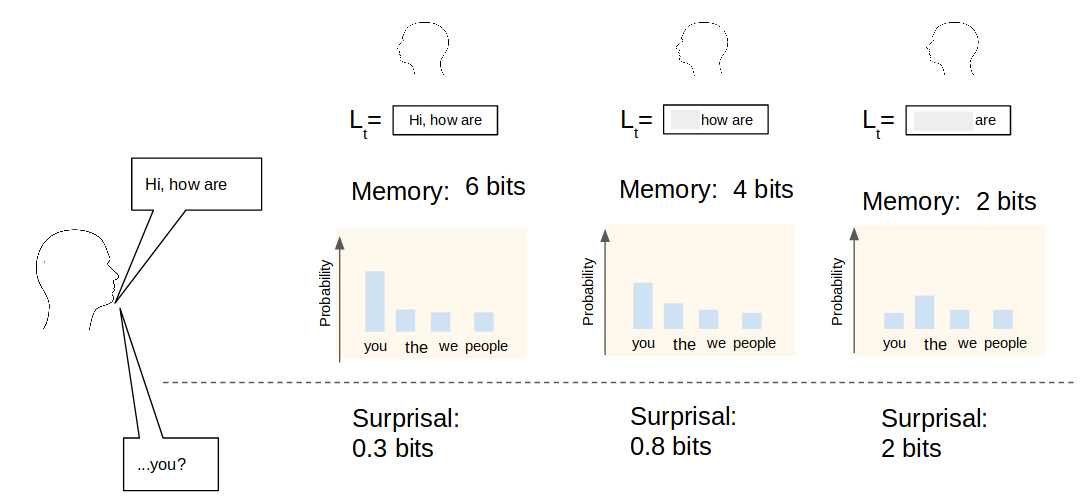
\includegraphics[width=0.9\textwidth]{figures-gdrive/communication.png}
	\caption{Memory and language comprehension. (1) A speaker produces a sequence of words. (2) A listener maintains a representation of the words received so far. The listener can represent these at higher (left) or lower (right) levels of precision. (3) Throughout communication, the listener generates probabilistic expectations about the next word. Higher precision of memory representations leads to more precise predictions. (4) When receiving the next word, the listener incurs surprisal depending on the predictions. Higher levels of fidelity in memory lead to lower surprisal on average. \jd{what do the numbers (1) (2) etc refer to? also: image is blurry, at least on my screen}\note{make reference to $L_t$ inside the caption. you and the surprisals visually better aligned. maybe can color-code? } \mhahn{problem suggests that memory has to be contiguous substrings}}
	\label{fig:communication}
\end{figure}

We begin developing our model by considering the process of language comprehension illustrated in Figure~\ref{fig:communication}, where the listener Alice is processing a stream of words uttered by an interlocutor Bob (Figure~\ref{fig:communication}). 

Experimental research has established three properties of online language comprehension: (1) listeners maintain some information about the words received so far in incremental memory, (2) listeners form probabilistic expectations about the upcoming words, and (3) words are easy to process to the extent that they are predictable based on a listener's memory of words received so far.

We formalize these three observations into postulates intended to provide a simplified picture of what is known about online language comprehension. Consider a listener comprehending a sequence of words $w_1, \dots, w_t, \dots, w_n$, at an arbitrary time $t$.
\begin{enumerate}
    \item Comprehension Postulate 1 (Incremental memory). At time $t$, the listener has an incremental \key{memory state} $m_t$ that contains her stored information about previous words. The memory state is given by a \key{memory encoding function} $M$ such that $m_t = M(w_{t-1}, m_{t-1})$.
    \item Comprehension Postulate 2 (Incremental prediction). The listener has a subjective probability distribution at time $t$ over the next word $w_t$ as a function of the memory state $m_t$. This probability distribution is denoted $P(w_t|m_t)$.
    \item Comprehension Postulate 3 (Linking hypothesis). Processing a word $w_t$ incurs difficulty proportional to the \key{surprisal} of $w_t$ given the memory state $m_t$:
    \begin{equation}
    \label{eq:lossy-surp}
    \text{Difficulty} \propto -\log P(w_t | m_t).
\end{equation}
\end{enumerate}
The claim that processing difficulty should be directly proportional to surprisal comes from \key{surprisal theory}. Surprisal theory is an established psycholinguistic theory that can capture reading time effects related to garden-path disambiguation \citep{hale2001probabilistic}, antilocality effects, and effects of syntactic construction frequency \citep{levy2008expectation}. Surprisal is a robust linear predictor of reading times in large-scale eye-tracking studies based on naturalistic text \citep{smith-effect-2013,goodkind-predictive-2018}.

Our expression differs from the usual formulation of surprisal theory in that we consider predictability based on a (potentially lossy or noisy) memory representation $m_t$, rather than predictability based on the true complete context $w_1, \dots, w_{t-1}$. The generalization to lossy memory representations is necessary to capture empirically observed effects of memory limitations on language processing, such as dependency locality and structural forgetting \citep{futrell-noisy-context-2017,futrell2019information}. For other ways of capturing effects of both memory limitations and probabilistic expectations, see \citet{demberg-incremental-2013} and \citet{rasmussen-2017-left}.

From the perspective of information theory, surprisal measures the \key{information content} of a word $w_t$ in context. The surprisal value can be interpreted as the amount of new information contained in the word $w_t$, measured in bits, given the listener's current memory state. If processing effort is indeed proportional to surprisal, then this means that the amount of work required to process a word scales linearly with the information content of that word. The idea that information-processing cost scales with information content is in line with recent theories of the cost of computation in neuroscience \citep{friston2010free,zenon2019information} and physics \citep{still2012thermodynamics}. 

In this work, we are interested in using theories of processing difficulty to derive predictions about languages as a whole, not about individual words or sentences. Therefore, we need a measure of the processing difficulty associated with a language as a whole. For this, we consider the \emph{average} surprisal per word in the language. We call this quantity the \key{average surprisal} of a language given a memory encoding function $M$, denoted $S_M$ and measured in bits.

Crucially, the listener's ability to predict upcoming words accurately depends on how much she remembers about previous words. As the precision of her memory increases, the accuracy of her predictions also increases, and the average surprisal $S_M$ for each incoming word decreases. Taking an information-theoretic perspective, we can think about the amount of information (measured in bits) about previous words stored in the listener's memory state. This quantity of information is given by the \key{entropy} of the memory state, denoted $H_M$:
\begin{equation}
    H_M \equiv - \sum_m P(m) \log P(m) \text{ bits},
\end{equation}
where the summation runs over all possible memory states $m$. As the listener stores more and more bits of information about the previous words her memory state, she can achieve lower and lower surprisal values for the upcoming words. This trade-off between memory and surprisal is the main object of study in this paper.

The \key{memory--surprisal trade-off curve} answers the question: for a given amount of information about previous words $H_M$ stored in the listener's memory state, what is the lowest achievable average surprisal $S_M$? Two example trade-off curves are shown in Figure~\ref{fig:examples}. In general, as the listener stores more information about previous words in her memory state, her lowest achievable average surprisal must go down. So the curve is always monotonically decreasing. However, the precise shape of the trade-off curve depends on the structure of the language being predicted. For example, Figure~\ref{fig:examples} shows how two processes might engender different trade-off curves, with Language $A$ allowing more favorable trade-offs than Language $B$. That is, for Language $A$, it is possible to achieve lower processing difficulty while investing less memory resources than in Language $B$.

\begin{figure}
\centering
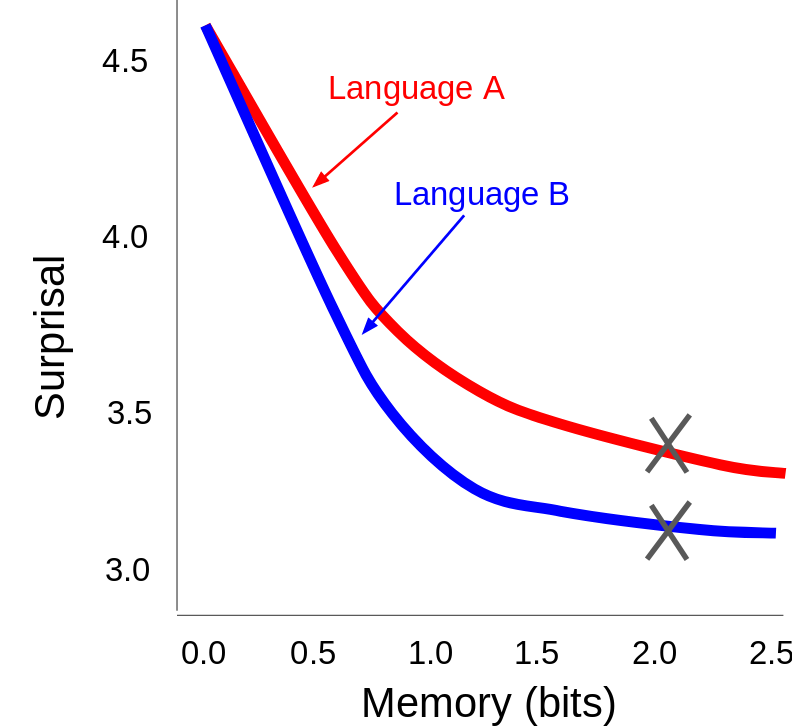
\includegraphics[width=0.5\textwidth]{figures-gdrive/tradeoff.png}
\caption{Example memory--surprisal trade-off curves for two languages, $A$ and $B$. While storing 2 bits of information in memory, a listener in Language $A$ can achieve an average surprisal of 3.5 bits, while a listener in Language $B$ can achieve an average surprisal of 3.25 bits. Language $B$ has a steeper memory--surprisal trade-off than Language $A$, and requires less memory resources to achieve the same level of processing difficulty.}
\label{fig:examples}
\end{figure}

\subsection{Main hypothesis}

Now that we have defined the memory--surprisal trade-off, we can precisely state the main hypothesis of this work:
\paragraph{Main hypothesis.}  Natural language is characterized by a distinctively steep memory--surprisal trade-off curve.

That is, natural language is memory-efficient in the sense that it is possible to achieve a low level of processing difficulty (average surprisal $S_M$) while storing a relatively small amount of information about previous words (entropy of memory $H_M$). We hypothesize that this structure is reflected both in the grammatical structure of languages and in usage preferences.

More specifically, in this paper we will claim that the word orders of natural languages are structured to maintain memory efficiency in this sense. Although we focus on word order in this paper, our hypothesis applies more generally, to any factors in grammar or usage which influence the memory--surprisal tradeoff.

\subsection{Formal definition of the memory--surprisal trade-off}

Here we provide the technical definition of the memory--surprisal trade-off curve and relate it to concepts from information theory, rate--distortion theory, and statistical complexity theory. 

Let $W$ be a stochastic process\footnote{We will use $W$ to represent languages, and we will construct $W$ to be stationary. Large natural language texts are known to be neither stationary nor ergodic \citep{}. However, we are interested in explaining grammatical properties of languages, which mostly involve constraints among words within sentences, not within large texts as a whole. Therefore, we will represent a language using a stochastic process consisting of repeated independent samples from a distribution over sentences. This stochastic process is both stationary and ergodic.} generating a stream of symbols called words, indexed as $w_1, \dots, w_t$.\footnote{We call these symbols words, but note that our mathematical treatment applies for \emph{any} decomposition of a sentence into a sequence of symbols---the symbols could represent phonemes, syllables, morphemes, words, phrases, etc.} Let $M$ be a memory encoding function. The \key{average surprisal} of the process $W$ under the memory encoding function $M$ is
\begin{equation}
    S_M &\equiv \lim_{t \rightarrow \infty} H[w_t | m_t],
\end{equation}
where the notation $H[\cdot | \cdot]$ indicates conditional entropy \citep[][p. 17]{cover2006elements}:
\begin{equation}
    H[w_t|m_t] \equiv -\sum_{w_t,m_t} P(m_t) P(w_t|m_t) \log P(w_t|m_t).
\end{equation}
The lowest possible average surprisal for $W$ that can be attained by any memory encoding function is called the \key{entropy rate} of $W$ \citep[][pp. 74--75]{cover2006elements}:
\begin{equation}
    \label{eq:entropy-rate}
    S_\infty \equiv \lim_{t \rightarrow \infty} H[w_t | w_1, \dots, w_{t-1}].
\end{equation}
 The entropy rate of a stochastic process is the irreducible unpredictability of the process: the extent to which a stream of symbols remains unpredictable even for a predictor with unlimited resources. 
 %Because $W$ is stationary and ergodic by construction, the limit in Eq.~\ref{eq:entropy-rate} is guaranteed to converge to a unique value. 
 The entropy rate of natural language text has been studied by \citet{shannon1951entropy}, \citet{takahira}, and \citet{bentz}. 
 The average surprisal $S_M$ can also be called a \key{cross entropy rate}. % TODO: Say something about convergence and uniqueness?
 Because the memory state $m_t$ is a function of the previous words $w_1, \dots, w_{t-1}$, we can prove by the Data Processing Inequality \citep[][pp. 34--35]{cover2006elements} that the entropy rate must be less than or equal to the average surprisal for any memory encoding function $M$:
\begin{equation}
    S_\infty \le S_M.
\end{equation}
If the memory state $m_t$ stores all information about the previous words $w_1, \dots, w_{t-1}$, then we have $S_M = S_\infty$.

% The "memory distortion" stuff below might be useful in an argument about the trade-off for the speaker.

In general, we can write the average surprisal $S_M$ as a sum of two non-negative terms,
\begin{equation}
    S_M = S_\infty + d_M,
\end{equation}
where $d_M$ is \key{memory distortion}: the extra surprisal incurred in addition to the unavoidable surprisal $S_\infty$, owing to the lossiness of the memory encoding function $M$. 
The memory distortion $d_M$ is formally a KL divergence:
\begin{equation}
    \label{eq:memory-distortion}
    d_M = \lim_{t \rightarrow \infty} D_{\text{KL}} [ p(w_t | w_1, \dots, w_{t-1}) || p(w_t | m_t)].
\end{equation}
Finding a memory encoding function $M$ to minimize $S_M$ is equivalent to minimizing the memory distortion $d_M$.

The average amount of information stored in the memory states $m_t$ is the entropy of the stationary distribution over memory states, $H_M$:
\begin{equation}
    \label{eq:memory-entropy}
    H_M \equiv H[m_t].
\end{equation}
The minimum value of $H_M$ that achieves $S_M = S_\infty$ is called the \key{statistical complexity} of the process $W$ \citep{feldman-measures-1998}. The statistical complexity of natural language has been studied by \citet{hahn2019neural}. We will be imposing bounds on $H_M$ and studying the resulting values of $S_M$. 

\begin{definition}
The \key{memory--surprisal trade-off curve} for a process $W$ is defined as the lowest achievable average surprisal $S_M$ for each value of $H_M$. Let $R$ denote an upper bound on the memory entropy $H_M$; then the memory--surprisal trade-off curve is given by
\begin{equation}
    \label{eq:ms-formal}
    D(R) \equiv \min_{M : H_M \le R} S_M.
\end{equation}
\end{definition}

The memory state $m_t$ is generally a lossy representation of the true context of words $w_1, \dots, w_{t-1}$, meaning that $m_t$ does not contain all the possible information about $w_1, \dots, w_{t-1}$. The mathematical theory of lossy representations is \key{rate--distortion theory}, a field within information theory \citep[for an overview and key results, see][pp. 301--347]{cover2006elements}. Rate--distortion theory studies curves of the form of Eq.~\ref{eq:ms-formal}, which quantify trade-offs between utility (`distortion') and information (`rate'). Our memory--surprisal trade-off curve is a distortion--rate curve, with $H_M$ as the rate and $S_M$ as the distortion. It differs from the typical curve studied in rate--distortion theory in that we define rate using entropy, rather than mutual information \citep[see][for a discussion of some of the consequences of this formulation]{strouse-deterministic-2017}. Our memory--surprisal curve is closely related to the \emph{predictive information bottleneck} introduced by \citet{still-information-2014} and studied by \citet{marzen-predictive-2016}; in particular, it is a version of the \emph{recursive information bottleneck} \citep[][\S 4]{still-information-2014}. 


\subsection{Information locality}

The shape of the memory--surprisal trade-off is determined in part by the grammatical structure of a language.
Some languages enable more efficient trade-offs than others by forcing a listener to store more bits in memory to achieve the same level of average surprisal.

Here, we will demonstrate that the memory--surprisal trade-off is optimized by languages with word orders exhibiting a property called \key{information locality}. Information locality means that words that depend on each other statistically are located close to each other in time. We will argue that information locality generalizes the well-known word order principle of dependency locality, which has been studied in psycholinguistics, corpus linguistics, and typology for decades \citep{rijkhoff-word-1986,hawkins-performance-1994,gibson-linguistic-1998,liu-dependency-2018,futrell-large-scale-2015,liu-dependency-2017,temperley-minimizing-2018}. 

We will make our argument by defining a lower bound on the memory--surprisal trade-off curve (Eq.~\ref{eq:ms-formal}). This lower bound represents an unavoidable cost associated with a certain level of memory usage $H_M$; the true average surprisal $S_M$ might be higher than this bound. 

Our argument will make use of a quantity called \key{mutual information}. Mutual information is the most general measure of statistical association between two random variables. The mutual information between two random variables $X$ and $Y$, conditional on a third random variable $Z$, is defined as:
\begin{align}
\label{eq:mi}
    I[X:Y|Z] &\equiv \sum_{x,y,z} P(x,y,z) \log \frac{P(x,y|z)}{P(x|z)P(y|z)} \text{ bits} \\
    &= H[X|Z] - H[X|Y,Z] \\
    &= H[Y|Z] - H[Y|X,Z].
\end{align}
Mutual information is always non-negative. It is zero when $X$ and $Y$ are conditionally independent given $Z$, and positive whenever $X$ gives any information that makes the value of $Y$ more predictable, or vice versa. 

We will study the mutual information structure of natural language sentences, and in particular the mutual information between words at certain distances in linear order. We define the notation $I_t$ to mean the mutual information between words at distance $t$ from each other, conditional on the intervening words:
\begin{align}
    I_t &\equiv I[w_t : w_0 | w_1, \dots, w_{t-1}] \\
    &= H[w_t | w_1, \dots, w_{t-1}] - H[w_t | w_0, \dots, w_{t-1}].
\end{align}
This quantity, visualized in Figure~\ref{fig:theorem}(a), measures how much predictive information is provided about the current word by the word $t$ steps in the past.
It is a statistical property of the language, and can be estimated from large-scale text data.

Equipped with this notion of mutual information at a distance, we can now state our theorem:
\begin{thm}\label{prop:suboptimal}(Information locality bound) For any positive integer $T$, let $M$ be a memory encoding function such that
\begin{equation}
\label{eq:memory-bound}
H_M \le \sum_{t=1}^T t I_t.    
\end{equation}
Then we have a lower bound on the average surprisal under the memory encoding function $M$:
\begin{equation}
\label{eq:surprisal-bound}
S_M \ge S_\infty + \sum_{t=T+1}^\infty I_t.
\end{equation}
\end{thm}
A formal proof, relying only on the stationarity of the stochastic process, is given in Appendix Section X. 

\paragraph{Interpretation} The theorem means that a predictor with limited memory capacity will always be affected by surprisal cost arising from long-term statistical dependencies of length greater than $T$, for some finite $T$. This is why we call the result `information locality': processes are easier to predict when most statistical dependencies are short-term (shorter than $T$). Below we explain in more detail how this interpretation matches the mathematics of the theorem.

The quantities in the theorem are illustrated visually in Figure~\ref{fig:theorem}. Eq.~\ref{eq:memory-bound} describes a memory encoding function which has enough capacity to remember the relevant information from at most $T$ words in the immediate past. The minimal amount of memory capacity which would be required to retain this information is the sum $\sum_{t=0}^T t I_t$, reflecting the cost of holding $I_t$ bits in memory for $t$ timesteps up to $t=T$. 

The information locality bound theorem says that the surprisal cost for this memory encoding function is at least $S_\infty + \sum_{t=T}^\infty I_t$ (Eq.~\ref{eq:surprisal-bound}). The first term $S_\infty$ is the entropy rate of the process, representing the bits of information in the process which could not have been predicted given any amount of memory. The second term $\sum_{t=T}^\infty I_t$ is the sum of all the relevant information contained in words \emph{more} than $T$ timesteps in the past (see Figure~\ref{fig:theorem}(b)). These correspond to bits of information in the process which \emph{could have} been predicted given infinite memory resources, but which were not, due to the limit on memory usage.

The theorem gives a lower bound on the memory--surprisal trade-off curve, meaning that there is no memory encoding function with memory capacity $H_M$ which achieves lower average surprisal than Eq.~\ref{eq:surprisal-bound}. In terms of psycholinguistics, if memory usage is bounded by Eq.~\ref{eq:memory-bound}, then processing cost of at least Eq.~\ref{eq:surprisal-bound} is inevitable.

\begin{figure*}
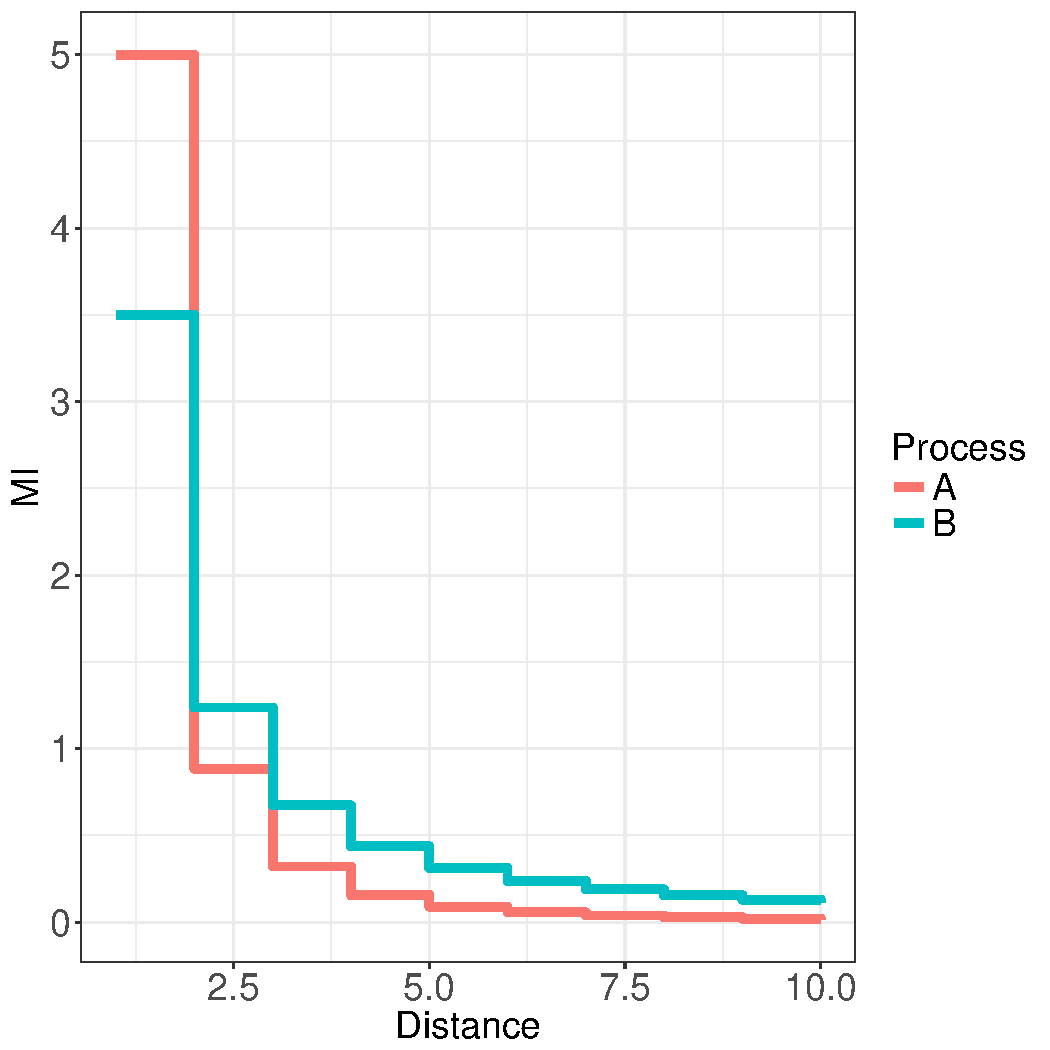
\includegraphics[width=0.45\textwidth]{figures/decay.pdf}
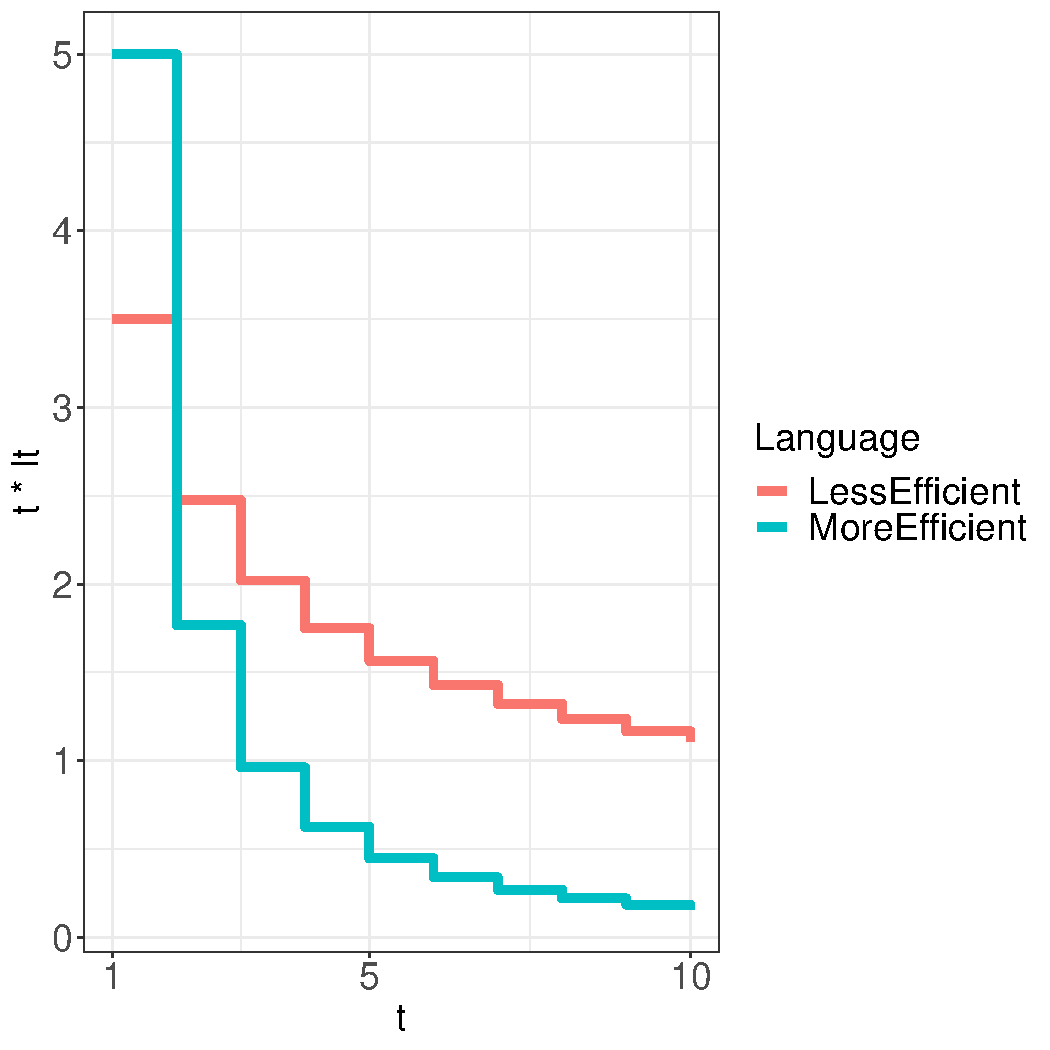
\includegraphics[width=0.45\textwidth]{figures/memory.pdf}
%
	\caption{Left: $I_t$ as a function of $t$, for two different processes. $I_t$ decays faster for the red process: Predictive information about the present observation is concentrated more strongly in the recent past. Left: $t \cdot I_t$ as a function of $t$ for the same processes. }\label{fig:basic}
\end{figure*}

\begin{figure}
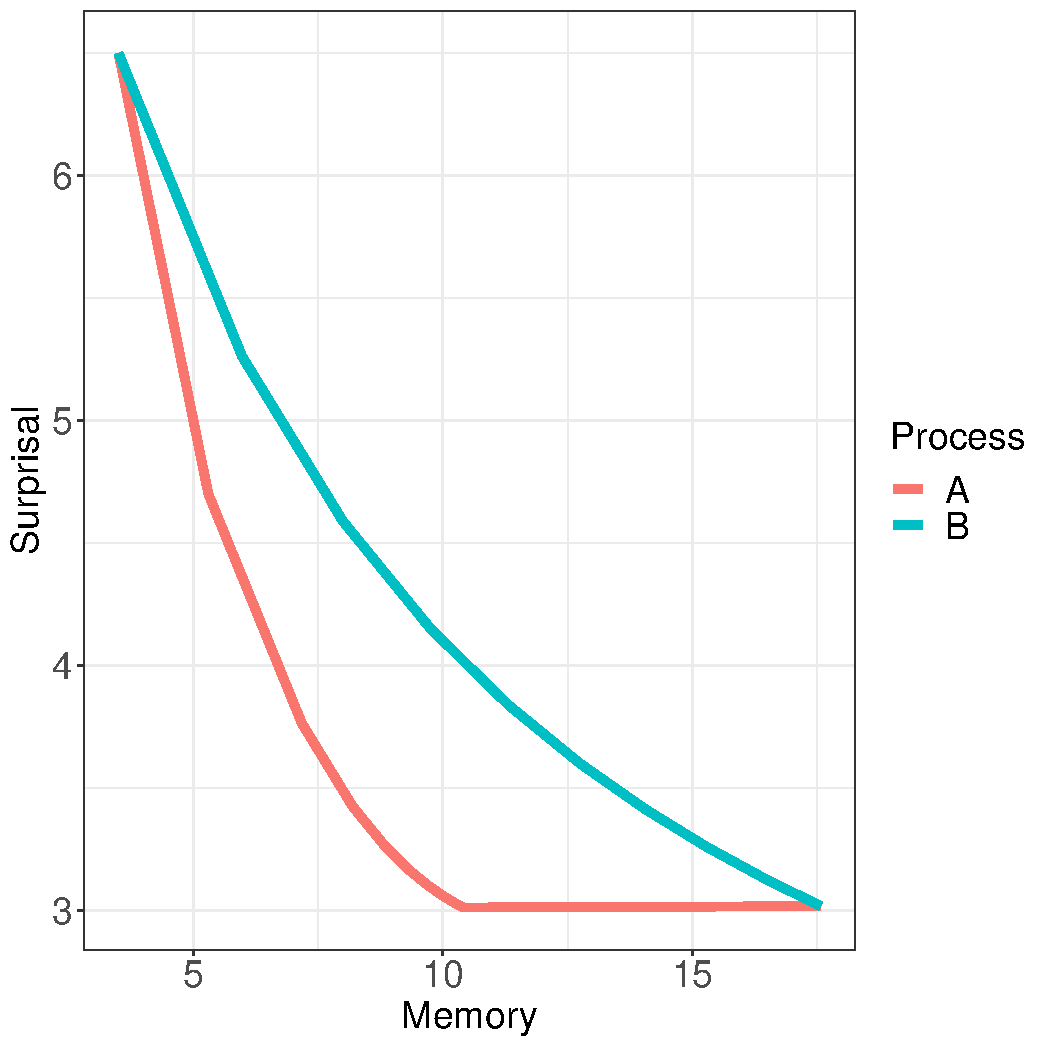
\includegraphics[width=0.45\textwidth]{figures/listener-tradeoff.pdf}
	\caption{Listener's memory-surprisal tradeoff for the two processes in Figure~\ref{fig:basic}. Recall that the red process had a faster decay of conditional mutual information. Correspondingly, this figure shows that a listener can achieve lower surprisal at the same level of memory load.}\label{fig:listener-tradeoff}
\end{figure}

Eq.~\ref{eq:memory-bound} means that maintaining long-term dependencies requires higher memory usage. Carrying the same amount of information over longer distances requires more memory; this fact is reflected in the factor $t$ inside each term of the sum. 
The result is that modeling long-term statistical dependencies is more costly in terms of memory usage than modeling shorter ones.
The information locality bound theorem demonstrates in a highly general way that language comprehension requires less memory resources when statistical dependencies are mostly short-term. 

Because processing long-term dependencies requires higher memory usage, the theorem also implies that a language will be easier to process when most of the predictive information about a word is concentrated close to that word in time---that is, when $I_t$ falls off rapidly as $t \rightarrow \infty$. When memory capacity is limited, then there must be some timescale $T$ such that a listener appears to be affected by excess surprisal arising from statistical dependencies of length greater than $T$. A language avoids such cost to the extent that it avoids dependencies with a time-span larger than $T$.

We illustrate the theorem in Figure~\ref{fig:basic}.
We consider two processes $A$ and $B$, where $I_t := 5t^{-1.5}$ for $A$ and $I_t := 3.5 t^{-2.5}$ for $B$.
The curves of $I_t$, as a function of the distance $t$, are shown in Figure~\ref{fig:basic} (left).
In both cases, $I_t$ converges to zero as $t$ grows to infinity. 
However, $I_t$ decays more quickly for Process A (red).
This means that predictive information about an observation is concentrated more strongly in the recent past.
In Figure~\ref{fig:basic} (right), we show $t\cdot I_t$ as a function of $t$.
Note that the area under the curve is equal to (\ref{eq:memory-bound}).
This area is smaller for the red process, as $I_t$ decays more quickly there.  


%\paragraph{Proof Sketch}
%An intuitive argument for the theorem goes as follows:
%For each bit of information that is held in memory, we count the number of timesteps from when it is first entered into memory to when it is forgotten.
%If a word $w_{T-t}$, $t$ steps in the past, contains one bit of information about the current word $w_T$, and if this information is not redundant with information in the intervening words, then this bit of information had to be maintained in memory for $t$ steps.
% This explains the factor $t$.

\paragraph{Relation with dependency locality}
Our information locality theorem says that \emph{statistical} dependencies should be short-term: that is, whenever one element of a sequence determines or predicts another element, those two elements should be close to each other in time. In contrast, linguistic theories of locality have typically focused on the time-span of \key{syntactic dependencies}: words which depend on each other to determine the meaning or the well-formedness of a sentence. The idea that syntactic dependencies should be short in word order, and that processing difficulty results when they are not, is called \key{dependency locality}. 

If statistical dependencies, as measured using mutual information, can be identified with syntactic dependencies, then that would mean that information locality is a generalization of dependency locality. \citet{futrell2019syntactic} gives theoretical and empirical arguments that this is so. They show that syntactic dependencies as annotated in dependency treebanks identify word pairs with especially high mutual information, and give a derivation showing that this is to be expected according to a formalization of the postulates of dependency grammar. The connection between mutual information and syntactic dependency has also been explored by \citet{}. 

\paragraph{Relation with previous derivations of information locality} A similar information locality result was established by \citet{futrell-noisy-context-2017}, who showed that if incremental memory is affected by progressively increasing noise, then (following the postulates above) processing difficulty increases when words with high pointwise mutual information are separated by large distances. Pointwise mutual information is the extent to which a \emph{particular value} predicts another value in a joint probability distribution. For example, if we have words $w_1$ and $w_2$ in a sentence, their pointwise mutual information is:
\begin{equation}
    \text{pmi}(w_1; w_2) \equiv \log \frac{P(w_2|w_1)}{P(w_2)}.
\end{equation}
Mutual information as we defined it in Eq.~\ref{eq:mi} is the \emph{average} pointwise mutual information over an entire probability distribution.

Our current result is both more general and more precise. Our theorem differs from \citet{futrell-noisy-context-2017} in three ways:
\begin{enumerate}
    \item \citet{futrell-noisy-context-2017} required an assumption that incremental memory is subject to decay over time. In contrast, we do not require any assumptions about incremental memory except that it has bounded capacity, or that retrieval operations have bounded capacity.
    \item Our result is a precise bound, whereas the previous result was an approximation based on neglecting higher-order interactions among words.
    \item Our result is about the fall-off of the mutual information between words, conditional on the intervening words. The previous result was about the fall-off of \emph{pointwise} mutual information between specific words, without conditioning on the intervening words.
\end{enumerate}

\paragraph{Relation with psycholinguistic theories of comprehension} 
Our result is couched in the language of surprisal theory \citep{hale2001probabilistic,levy2008expectation,hale2016information}, but the memory--surprisal curve reflects fundamental information-theoretic trade-offs that must apply in any theory. In particular, we have made no assumptions about the architecture of incremental memory, and so our result is general across all such architectures: there is no physically realizable memory architecture that can violate the bound in our theorem. In particular, we emphasize that memory representations do not have to be rational or optimal for our bound to hold.

In some psycholinguistic theories, memory-related difficulty arises not because of a bound on memory capacity, but rather because of difficulties involved in retrieving information from memory \citep{}. We are able to prove an analogous theorem that applies to such theories: see General Discussion for an extension of our analysis to the case involving a short-term memory (STM) with unbounded capacity, a working memory (WM) with limited capacity, and cost associated with communication between WM and STM. Essentially, the constraint on the the memory state in our theorem above can be re-interpreted as a constraint on the capacity of a communication channel linking STM to WM. In particular, this result constrains average surprisal for memory models based on cue-based retrieval such as the ACT-R model of \citet{lewis-activation-based-2005}.

While we have proven a general relationship between memory capacity and average surprisal, psycholinguistic theories may differ on whether average surprisal $S_M$ really is the right predictor of processing difficulty for humans. That is, our Linking Hypothesis is not an explicit part of all existing psycholinguistic theories.

We argue that any realistic theory of sentence processing must include surprisal as at least a \emph{component} of the cost of processing a word, even if it is not explicitly stated as such. More formally, we argue that processing difficulty for a word $w_t$ must at least be given by $k (-\log P(w_t |m_t)) + R$, with $k$ a scaling factor giving the relative contribution of surprisal to processing cost, and $R$ representing all other factors. The scaling factor $k$ may be small, but it cannot be zero, for both empirical and theoretical reasons. Empirically, surprisal makes a well-documented and robust contribution to processing difficulty in empirical studies of reading times and event-related potentials \citep{smith2013effect,frank2016erp}. Theoretically, surprisal may represent an irreducible thermodynamic cost incurred by any information processing system \citep{brillouin,still2012thermodynamic,zenon2019information}, and there are multiple converging theoretical arguments for why it should hold as a cost in human language processing in particular \citep{levy2013memory}. See General Discussion for a more detailed discussion how how average surprisal can describe processing cost in ACT-R models of sentence processing.

\paragraph{Are distant words forgotten?} Our theorem shows that a listener will inevitably be affected by surprisal cost corresponding to dependencies longer than some timescale $T$. However, it does not necessarily imply that a listener forgets words beyond some amount of time $T$ in the past. An optimal listener may well decide to remember words more distant than $T$, but in order to stay within the bounds of memory, she can only remember words from beyond $T$ at the cost of forgetting some information about words closer than $T$.
The Information Locality Lower Bound still holds, in the sense that the long-term dependency will cause processing difficulty, even if the long-term dependency is not itself forgotten.
See SI Appendix Section X for a mathematical example illustrating this phenomenon.
%\rljf{TODO: This needs to be clarified. This is basically about the non-tightness of the bound.}

\mhahn{Do we also want to expound on what `bits of memory' means? E.g., how this could be instantiated in different mechanistic models or grammar formalisms. Also, we can make clear that capacity bounds do not have to mean bounds on the number of `items' in memory, but also, e.g., bounds on the precision with which these are encoded or utilized.}

\paragraph{Computing the lower bounds}
The theorem allows us to estimate numerical values for the lower bounds on the average surprisal associated with each amount of memory capacity for a language.
All that is required is to estimate the quantities $I_t$.
The quantities $I_t$ can be estimated as the difference between the cross-entropy of language models that have access to the last $t-1$ or $t$ words.
That is, if we have a $t$th-order Markov model with average surprisal
\begin{equation}
    S_t = H[w_t | w_0, \dots, w_{t-1}]
\end{equation}
and a $(t-1)$th-order Markov model with average surprisal
\begin{equation}
    S_{t-1} = H[w_t | w_1, \dots, w_{t-1}],
\end{equation}
then we can calculate $I_t$ straightforwardly:
\begin{align}
    I_t &= I[w_t : w_0 | w_1, \dots, w_{t-1}] \\
    &= S_{t-1} - S_t.
\end{align}
We can use LSTMs to fit $t$th-order Markov models for various values of $t$ to natural language sentences, and then use the resulting $S_t$ values to calculate lower bounds on the memory--surprisal trade-off curve using the theorem by tracing out $t=1, 2, \dots$.



\begin{figure}
	(a)
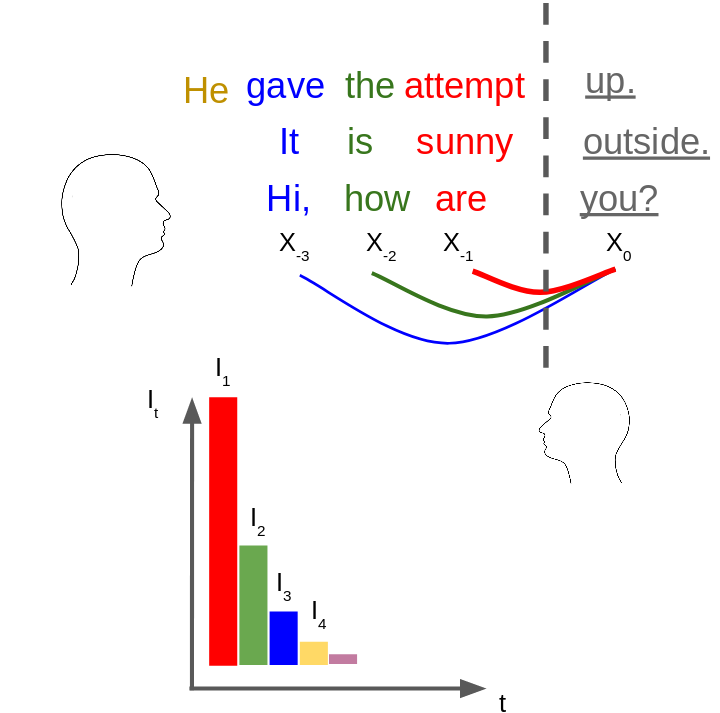
\includegraphics[width=0.4\textwidth]{figures-gdrive/mi-distance.png}
	(b)
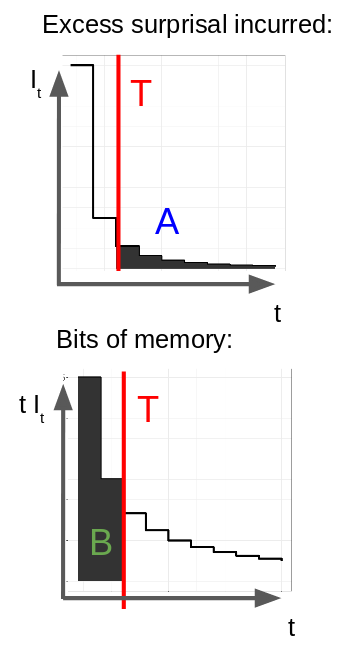
\includegraphics[width=0.2\textwidth]{figures-gdrive/theorem.png}
	\caption{
		(a) Conditional mutual information $I_t$ captures how much predictive information about the next word is provided, on average, by the word $t$ steps in the past.
		(b) Here we illustrate our theoretical result. We plot $I_t$ (top) and $tI_t$ (bottom) as functions of $t$. A listener using $B$ bits memory (bottom) to represent prior observations will incur at least $A$ bits of extra surprisal beyond the entropy rate (top). \note{there is t and T. COnfusing}
		(c) \jd{FILL OUT} \note{make the colors in (c) difefrenfr from this in (b). Do want to make clear what the mapping from (b) to (c) is. Maybe can even have a pair of the two (b) curves, and then show what they map on.}
}\label{fig:theorem}
\end{figure}



\subsection{Memory--surprisal trade-off in language production}

An analogous memory--surprisal trade-off exists in language production. In this case, the trade-off arises from the minimization of error in production of linguistic sequences. That is, given a \key{competence language} (a target distribution on words given contexts), a speaker tries to produce a \key{performance language} which is as close as possible to the competence language. The performance language operates under memory constraints, so the performance language will diverge from the competence language due to production errors. As a speaker has more and more incremental memory about what she has already produced, she is able to produce linguistic sequences with less error, thus reducing the divergence between the performance language and the competence language. The reduction of this competence--performance divergence is formally equivalent to the minimization of average surprisal from Section~\ref{sec:listener-tradeoff}.

% TODO maybe cite some Karl Lashley stuff? Maryellen MacDonald? Shota Momma?

We derive the existence of this trade-off from the following postulates about language production. Let the competence language be represented by a stationary stochastic process, parameterized by a probability distribution $p(w_t | \mathbf{w_{<t}})$ giving the conditional probability of any word $w_t$ given an unbounded number of previous words. Our postulates describe a speaker who tries to find a performance language $q(w_t|m_t)$ to match the the competence language using incremental memory representations $m_t$:

\begin{enumerate}
    \item Production Postulate 1 (Incremental memory). At time $t$, the speaker has an incremental \key{memory state} $m_t$ that contains (1) her stored information about previous words that she has produced, and (2) information about her production target. The memory state is given by a \key{memory encoding function} $M$ such that $m_t = M(w_{t-1}, m_{t-1})$. This memory encoding function may differ from the one used in comprehension.
    
    \item Production Postulate 2 (Production policy). At time $t$, the speaker produces the next word $w_t$ conditional on her memory state by drawing from a probability distribution $q(w_t | m_t)$. We call $q$ the speaker's \key{production policy}.
    
    \item Production Postulate 3 (Minimizing divergence). The production policy $q$ is selected to minimize the Kullback-Leibler divergence to a target competence language $p(w_t|\mathbf{w}_{<t})$. We call this divergence the \key{competence--performance divergence} under the memory encoding function $M$ and the production policy $q$. It measures the extent to which the produced language differs from the target language:
    \begin{align}
    \label{eq:comp-perf-div}
    d^q_M &\equiv D_{\text{KL}} [ p(w_t|\mathbf{w_{<t}}) || q(w_t|m_t) ] \\
        &= \sum_{\mathbf{w_{\le t}}} p(\mathbf{w_{\le t}}) \log \frac{p(w_t | \mathbf{w_{<t}})}{q(w_t|m_t)}.
    \end{align}
    The production policy is then the solution to the functional minimization problem:
    \begin{equation}
        \mathop{\text{minimize }}_{q(w_t|m_t)} d^q_M.
    \end{equation}
\end{enumerate}

Completing the link with the memory--surprisal trade-off in comprehension, we note that when the production policy $q(w_t|m_t)$ is selected to minimize the competence--performance divergence $d^q_M$, then this divergence becomes equal to the memory distortion $d_M$ discussed above in the context of comprehension costs. Therefore, under these postulates, the Information Locality Bound Theorem will apply in production as well as comprehension. This means that languages that exhibit information locality can be produced with greater accuracy given limited memory resources.

Although the memory--surprisal trade-off is mathematically equivalent between comprehension and production, its psycholinguistic interpretation is different. In the case of language comprehension, the trade-off represents excess processing \emph{difficulty} arising due to memory constraints. In the case of language production, the trade-off represents \emph{production error} arising due to memory constraints. When memory is constrained, then the speaker's productions will diverge from her target language. And as memory is more and more constrained, this divergence will increase more and more. The degree of divergence is measured in the same units as surprisal, hence the formal equivalence between the listener's and speaker's memory--surprisal trade-offs. 









%\begin{figure}
%	\begin{center}
%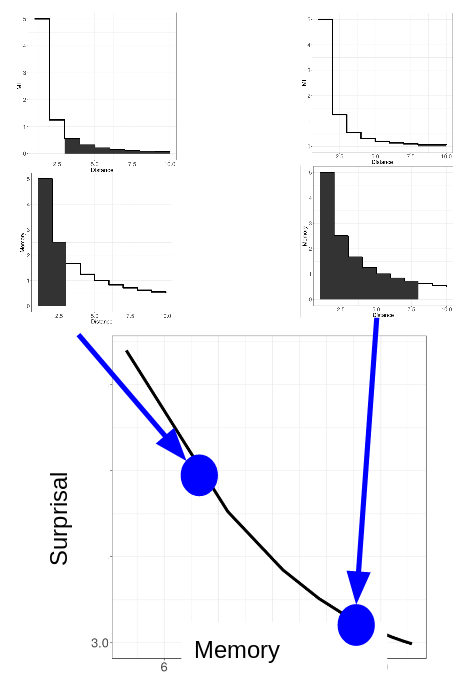
\includegraphics[width=0.45\textwidth]{figures/interpolate-curve.png}
%\end{center}
%	\caption{Estimating memory-surprisal tradeoff using the Theorem: We trace out the memory and surprisal values for all $T=1, 2, ...$, and linearly interpolate the curve.}\label{fig:interpolate}
%\end{figure}




%\begin{figure}
%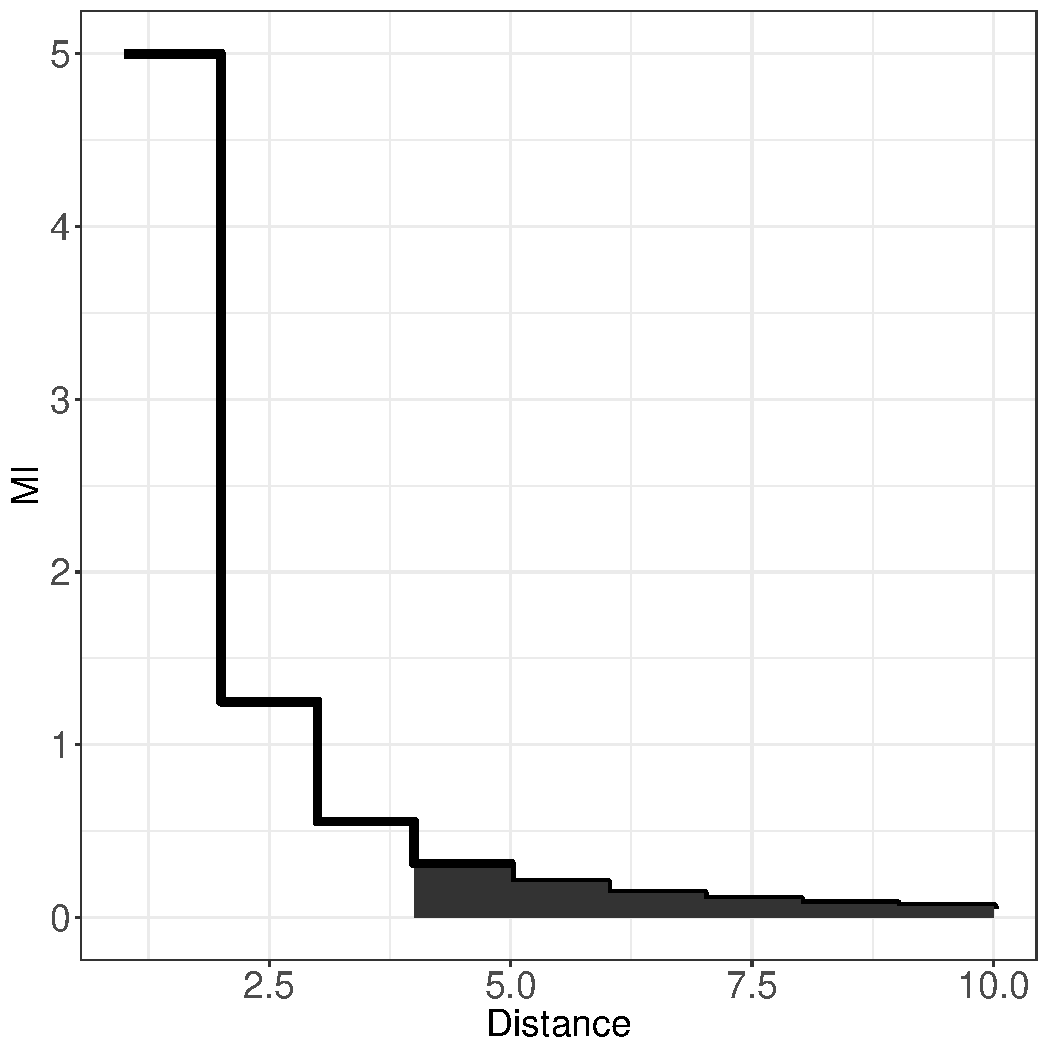
\includegraphics[width=0.45\textwidth]{figures/add-surp.pdf}
%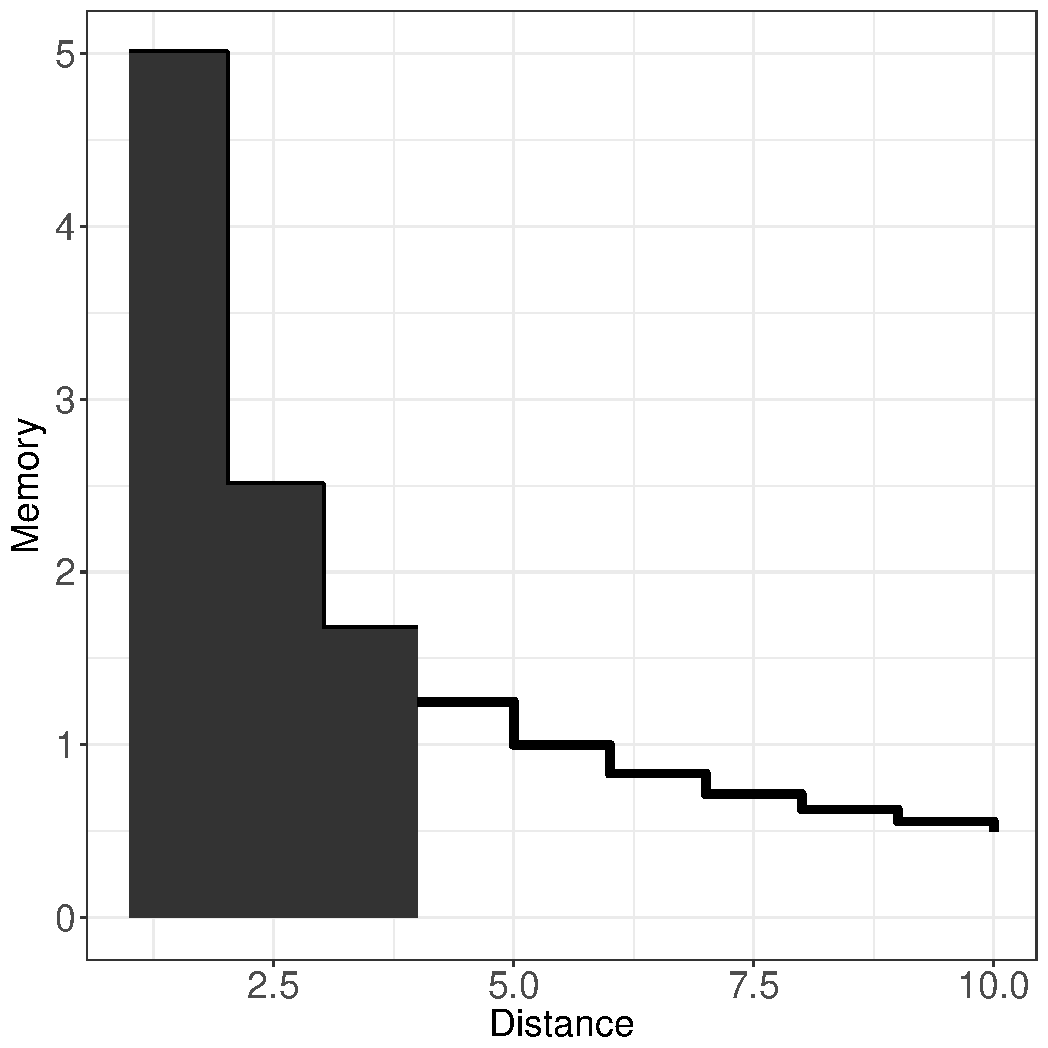
\includegraphics[width=0.45\textwidth]{figures/lower-mem.pdf}
%	\caption{Illustration for Proposition~\ref{prop:suboptimal}. Listeners can trade off memory and surprisal: A listener only investing memory of the amount given by the black area on the right will incur at least the black area on the left in additional surprisal. In the given example, $T=4$. By varying $T$, the two areas describe the listener's memory-surprisal tradeoff curve.}\label{fig:listener-tradeoff-decay}
%\end{figure}





%\subsection{Formal Analysis and Proofs}













